%%%%%%% Damit fangen wir nächste Woche an %%%%%%%%
\newpage
\newpage
\section[Einführung in die Gebietsintegrale]{Mehrdimensionale Integrale}
\subsection{Theoretisches Baukasten}
Um uns mit mehrdimensionalen Integralen zu beschäftigen, müssen wir zuerst gewisse theoretische Begriffe einführen.
\begin{Def}{Charakteristische Funktion}
Sei $A\subseteq \R^n$. Die charakteristische Funktion \textit{oder auch} \red{Indikatorfunktion} der Teilmenge $A$ ist die Funktion
$$1_A:\R^n \rightarrow \R \mbox{ mit } x\rightarrow \begin{cases}1, x\in A \\
0, x\notin A\end{cases}$$
\end{Def}
\begin{Def}{Quader}
Ein \red{Quader} $Q\subseteq \R^n$ ist das Produkt $I_1\times \cdots \times I_n$ von $n$ beschränkten, nicht-leeren Intervallen $I_\mu \subseteq \R$.
\end{Def}
\begin{Beispiel}{Quader in $\R^1$}
Quader in $\R^1$ sind also die Intervale $(a,b)$, $[a,b]$, $(a,b]$ und $[a,b)$. \\
\end{Beispiel}
\begin{Def}{Volumen eines Quaders}
Das (n-dimensionale) Volumen eines solchen Quaders ist die nicht-negative reelle Zahl
$$v(Q)=v_n(Q)=\prod_{\mu = 1}^n |I_\mu|=\prod_{\mu = 1}^n (b_\mu - a_\mu)$$
\end{Def}
\begin{Def}{Treppenfunktion}
Eine Funktion $\varphi:\R^n \rightarrow \C$ heißt \red{Treppenfunktion auf $\R^n$}, wenn es endlich viele paarweise \textbf{disjunkte} Quader gibt, sodass
\begin{enumerate}[a)]
    \item die Funktion $\varphi$ auf jedem Quader $Q_k$ konstant ist,
    \item $\varphi(x)=0$ für alle $x$ außerhalb von Quadern.
    \end{enumerate}
Außerdem lassen sich Treppenfunktionen als endliche Linearkombination charakteristischer Funktionen von disjunkten Quadern schreiben
$$\varphi=\sum_{k}c_k 1_{Q_k} \mbox{ mit $c_k\in \C$ und $Q_k$ ist ein Quader}$$ 
\end{Def}
Wir kommen nun zu den sehr wichtigen Begriff der Hüllreihen.
\begin{Def}{Hüllreihe}
Gegeben sei $f:\R^n\rightarrow\C\cup \{\infty\}$. Eine \red{Hüllreihe} zu $f$ ist eine Reihe
$$\Phi=\sum_{k=1}^\infty c_k1_{Q_k} \mbox{ mit $c_k\in \R$}$$
wobei $Q_k$ \textbf{offene} Quader im $\R^n$ sind und für jedes $x\in\R^n$ gilt
$$|f(x)|\leq \Phi(x) = \sum_{k=1}^\infty c_k1_{Q_k}(x)$$
Der \red{Inhalt} der Hüllreihe ist definiert als
$$I(\Phi) = \sum_{k=1}^\infty c_k v(Q_k)$$
\end{Def}

\begin{Beispiel}{Folge von Hüllreihen}
Seien $a, k\in \R$ und $f:\R\rightarrow\R$ definiert als $f(x)=\begin{cases}0, x\neq a && k, x=a\end{cases}$. Wir sollen zu dieser Funktion eine Folge von Hüllreihen, $\Phi_n$, konstruieren, die gegen Null konvergiert. \\
Wir wissen, dass $\Phi = \sum_{k=1}^\infty c_k 1_{Q_k}$, aber auch, dass $c_k=0$ für jeden Quader außer für die, in denen sich $a$ befindet (da ist $c_k=k$). Wir können Hüllen als Intervale bilden und bekommen die Hüllreihe:
$$A_n=[a-\frac{1}{n}, a+\frac{1}{n}]$$
Die Inhalte dieser Hüllreihe gehen gegen 0
$$\lim_{n\rightarrow\infty}I(A_n)=\lim_{n\rightarrow\infty} a+\frac{1}{n}-(a-\frac{1}{n})=\lim_{n\rightarrow\infty}\frac{2}{n}=0$$
Wir haben nun erfolgreich eine Folge von Hüllreihen konstruiert
$$\Phi_n=\sum_{n=1}^\infty A_n$$
\red{muss noch verifiziert werden}
\end{Beispiel}
\begin{Beispiel}{Hüllreihe einer Funktion}
            \begin{center}
    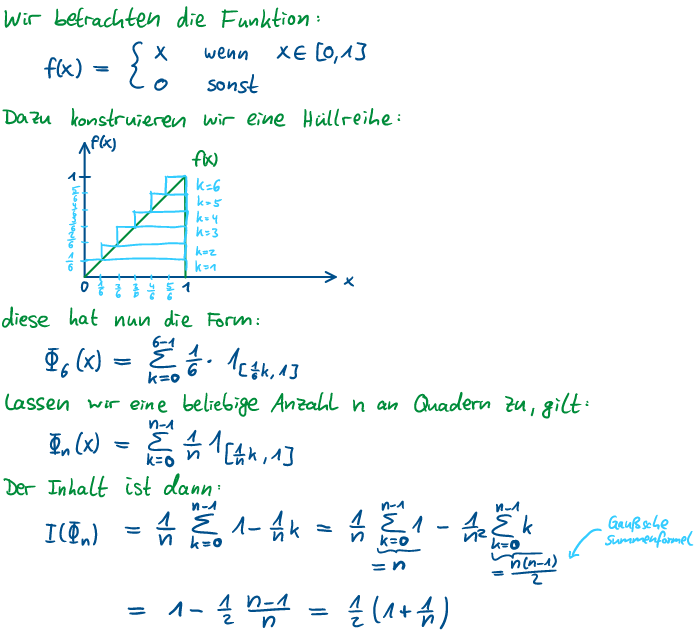
\includegraphics[width=0.80\textwidth]{Dateien/Robin_Hullreihen1.png}
    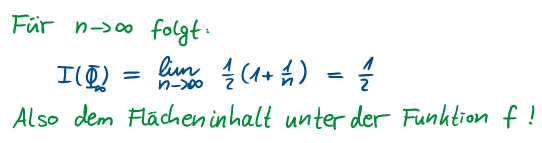
\includegraphics[width=0.80\textwidth]{Dateien/Robin_Hullreihen2.png}
\end{center}
\end{Beispiel}
\begin{Def}{$L^1$-Halbnorm}
Unter der \red{$L^1$-Halbnorm} von $f:\R^n\rightarrow\C\cup \{\infty\}$ versteht man das Infimum
$$||f||_1=\inf\{I(\Phi) |\mbox{ $\Phi$ Hüllreihe zu $f$} \}=\int |f|dx$$
\end{Def}
\begin{Satz}{Satz}{Eigenschaften einer Halbnorm}
Für die Funktionen $f_1, f_2: \R^n\rightarrow \C\cup\{\infty\}$ und ein $c\in\C$ gilt
\begin{enumerate}
\item $||c\cdot f||_1 = |c|\cdot ||f||_1$
\item $|f_1| \leq |f_2|  \implies ||f_1||_1 \leq ||f_2||_2$
\item $||\sum_{k=1}^\infty |f_k| ||_1\leq \sum_{k=1}^\infty ||f_k||_1$
\end{enumerate}
\end{Satz}
\newpage
\subsection{Lebesgue-Integral}
Mit den obigen theoretischen Werkzeug können wir nun endlich das Lebesgue-Integral definieren.
\begin{Def}{Lebesgue-Integral}
Eine Funktion $f:\R^n\rightarrow\C\cup\{\infty\}$ heißt \red{Lebesgue-integrierbar} über $\R^n$, wenn es eine Folge von Treppenfunktionen $\varphi_k$ gibt mit
$$\lim_{k\rightarrow \infty}||f-\varphi_k||_1=0$$
In diesem Fall schreiben wir das \red{Lebesgue-Integral}
$$\int fdx = \int f(x) d^nx = \int_{\R^n} f(x)dx = \lim_{k\rightarrow\infty} \varphi_k(x)dx\in\C$$
\end{Def}
\begin{Satz}{Satz}{Bedingte Gleichheit der Riemann und Lebesgue Integrale}
Sei $A=[a,b]$ ein kompaktes Intervall und $f$ eine über $A$ Riemann-integrierbare Funktion. Dann ist $f$ über $A$ Lebesgue-integrierbar und das Lebesgue-Integral und das Riemann-Integral sind gleich.
\end{Satz}
Der folgende zwei Sätze sind sehr wichtig in der Theorie der Gebietsintegrale. Im Skript stehen der kleiner und großer Satz von Fubini, wir schreiben hier aber die allgemeine Version aus T. Arens, also guckt euch auch das Skript nochmal an.
\begin{Satz}{Satz}{Kleiner Satz von Beppo Levi}
Sei $f:\R^n\rightarrow \R\cup \{\infty\}$ und sei $(\varphi_k)$ eine monoton wachsende oder fallende Folge von Treppenfunktionen, so dass
\begin{enumerate}[a)]
    \item $(\varphi_k)$ punktweise gegen $f$ konvergiert
    \item die Folge ($\int \varphi_k dx$) der Integrale der Treppenfunktionen beschränkt ist.
    Dann ist $f$ integrierbar und es gilt
    $$\int f dx=\lim_{k\rightarrow \infty}\int \varphi_k dx$$
\end{enumerate}
\end{Satz}
\begin{Satz}{Satz}{Satz von Fubini}
Sind $I\subseteq R^p$ und $J\subseteq R^q$ (möglicherweise unbeschränkte) Quader sowie $f\in L(Q)$ eine auf dem Quader $Q=I\times J \subseteq R^{p+q}$ integrierbare (oder mindestens stetig beschränkte) Funktion, so gibt es Funktionen $g\in L(I)$ und $h\in L(J)$ mit
$$g(x)=\int_J f(x,y) dy \mbox{ für fast alle $x\in I$}$$
$$h(y)=\int_I f(x,y)dx \mbox{ für fast alle $y\in J$}$$
Ferner ist 
$$\int_R f(x,y) d(x,y) = \int_I\int_J f(x,y) dy dx = \int_I g(x) dx$$
$$=\int_J\int_I f(x,y) dx dy = \int_J h(y) dy$$

\end{Satz}
\red{Wichtig!} Um den Satz von Fubini anwenden zu können, muss folgendes erwähnt werden:
\begin{itemize}
    \item $Q$ ist kompakt oder offen und beschränkt und
    \item $f$ ist stetig.
\end{itemize}
\begin{Beispiel}{Kompakte Kreissscheibe}
    Gegeben ist die kompakte Kreisscheibe:
    $$K=\overline{B_r(0)}=\{(x,y)\in\R^2| x^2+y^2\leq r^2\}$$
    Wir wollen nun das Integral
    $$\int_K 1 d(x,y)$$
    berechnen. Dazu stellen wir fest:
    \begin{enumerate}
        \item K ist kompakt
        \item $f(x,y)= 1$ ist stetig und beschränkt
        \item Die Menge $K_y$ lautet:
        $$K_y=\{x\in \R| (x,y)\in K\}=\{ x\in \R | x^2+y^2 \leq r^2\}$$
        $$= \{x\in \R | |x| \leq \sqrt{r^2-y^2}\}=[-\sqrt{r^2-y^2}, \sqrt{r^2-y^2}]$$
    \end{enumerate}
    Man erkennt leicht, dass $K_y\neq \emptyset$ für $y\in [-r, r]$. Somit erhalten wir:
    \begin{equation}
        F(y)=\begin{cases}\int_{K_y} 1dx & \mbox{ für $y\in [-1, 1]$} \\0 & \mbox{sonst}\end{cases}
    \end{equation}
    und damit nach dem Satz von Fubini:
    $$\int_K 1 d(x,y) = \int_\R F(y) dy = \int_{[-1,1]}[\int_{[-\sqrt{r^2-y^2}, \sqrt{r^2-y^2}]} 1dx]dy= \int_{-1}^{1} [\int_{-\sqrt{r^2-y^2}}^{\sqrt{r^2-y^2}} 1dx]dy=\pi r^2$$
    Eine nützliche Integrationsregel \red{$\int \sqrt{a^2-x^2}=\frac{1}{2}(a^2\sin^{-1}(\frac{x}{a})+x\sqrt{a^2-x^2})+c$}.
\end{Beispiel}
\begin{Beispiel}{Anwendung vom Satz von Fubini}
Wir wollen auch für eine kompliziertere Funktion, aber noch stets definiert auf einem Rechteck, die interierten Integrale berechnen. Dazu betrachten wir $R=(0,\frac{\pi}{2})\times (0,\frac{\pi}{2}$ und die Funktion $f:R\rightarrow \R$, die durch
$$f(x)=\sin(x_1+2x_2), \mbox{ $x=(x_1,x_2)\in R$}$$
gegeben ist.
\begin{center}
    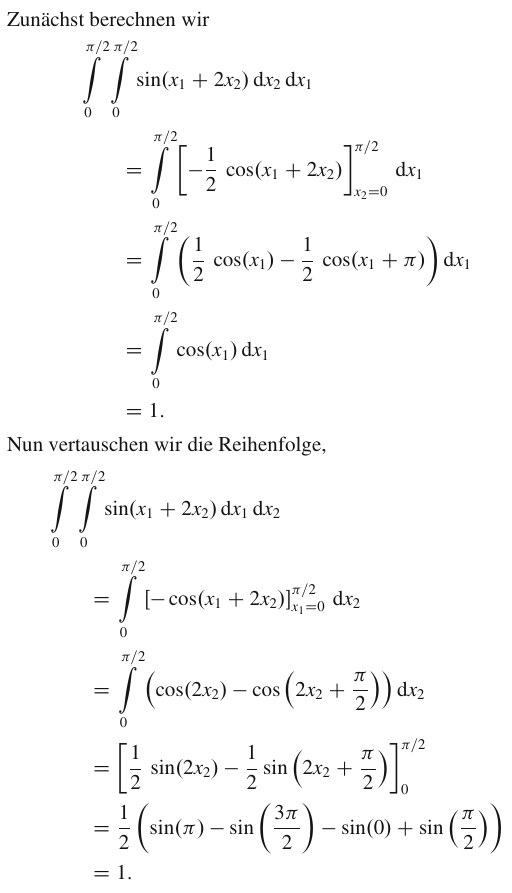
\includegraphics[width=.6\textwidth]{Dateien/Fubini1.png}
\end{center}
\end{Beispiel}
\begin{Beispiel}{Fubini ist nicht immer anwendbar}
\begin{center}
    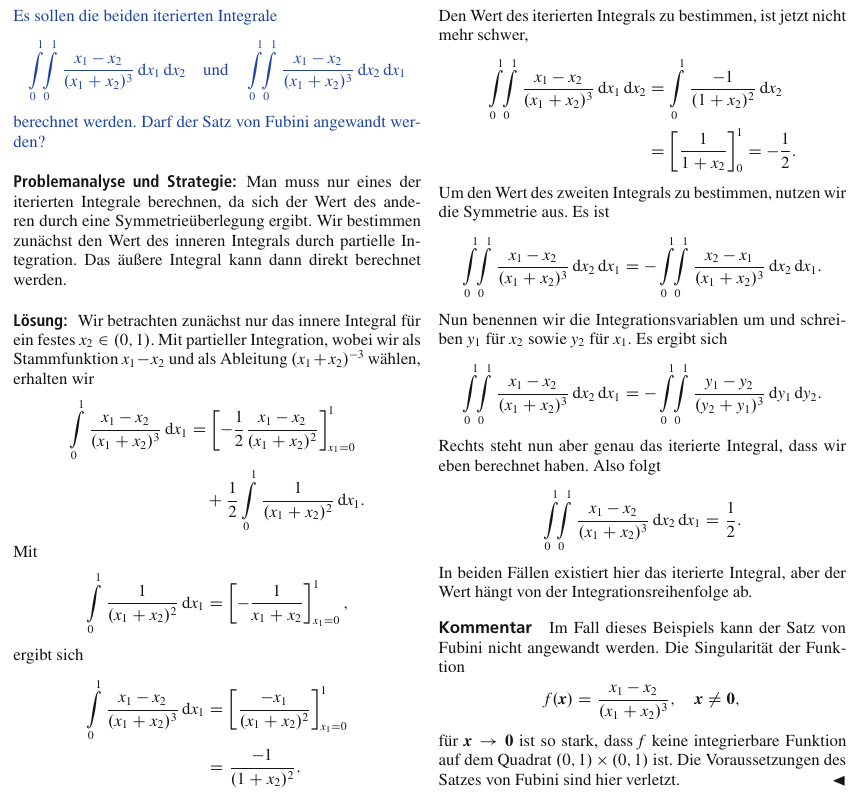
\includegraphics[width=\textwidth]{Dateien/Fubini2.png}
\end{center}
\end{Beispiel}
\newpage
\subsection{Volumina und Nullmengen}

Wir beginnen dieses wichtige Thema mit sehr theoretischen Konzepten, die uns dann ermöglichen die Maßtheorie zu verstehen. So manche Begriffe werden in der Funktionalanalysis in MfP4 nochmal vorkommen.
\begin{Def}{Grundmenge und $\sigma$-Algebra}
Eine \red{Grundmenge} (auch Universum), $\Omega$, bezeichnet in der Mathematik eine Menge aus allen in einem bestimmten Zusammenhang betrachteten Objekten. \\
Eine Menge $\mathcal{A}$ von Teilmengen einer Grundmenge $\Omega$ heißt \red{$\sigma$-Algebra}, wenn
\begin{itemize}
    \item $\Omega \in \mathcal{A}$
    \item Für jede Menge $A\in \mathcal{A}$ gilt $\Omega / A\in \mathcal{A}$
    \item Abzählbare Vereinigungen von Mengen $A_i\in \mathcal{A}$ sind wieder in $\mathcal{A}$
\end{itemize}
\end{Def}
\begin{Beispiel}{Kleinste und größte $\sigma$-Algebra}
Für jede beliebige Menge $\Omega$ ist $\{\emptyset, \Omega\}$ die kleinste und die Potenzmenge $P(\Omega)$ die größtmögliche $\sigma$-Algebra mit $\Omega$ als Grundmenge.
\end{Beispiel}
\begin{Def}{Maß}
Sei $\mathcal{A}$ eine $\sigma$-Algebra. Eine Funktion $\mu: \mathcal{A}\rightarrow[0,\infty]$ heißŧ ein \red{Maß} auf $\mathcal{A}$, wenn
\begin{itemize}
    \item $\mu(\emptyset)=0$,
    \item $\sigma$-Additivität, also $\mu(\cup_{n=1}^\infty A_n)=\sum_{n=1}^\infty \mu(A_n)$.
\end{itemize}
Außerdem wird das Tripel $(\Omega, \mathcal{A}, \mu)$ \red{Maßraum} gennant.
\end{Def}
\begin{Beispiel}{Borelsche $\sigma$-Algebra}
Die \red{borelsche $\sigma$-Algebra} ist eine $\sigma$-Algebra, die alle Mengen enthält, denen man naiverweise ein Volumen oder eine Wahrscheinlichkeit zuordnen will, schließt aber Negativresultate aus. \\
Bezüglich der borelschen $\sigma$-Algebra sind alle stetigen Funktionen immer messbar.
\end{Beispiel}
\begin{Def}{$\sigma$-Kompaktheit}
    Eine Menge $A\subseteq \R^n$ heißt \red{$\sigma$-kompakt}, wenn sie eine Vereinigung abzählbar vieler kompakter Menger ist.
\end{Def}
Nun kommt eine sehr wichtige Definition.
\begin{Def}{Lebesgue-Messbarkeit}
Eine Menge $A\subseteq \R^n$, falls die konstante Funktion über $A$ integrierbar ist.
$$v(A)=v_n(A)=\int_A 1dx$$
\end{Def}
\begin{Def}{Figur und Ausschöpfung}
Eine Vereinigung endlich vieler Quader $Q_i\subseteq \R^n$ der Form $A=Q_1\cup Q_2 \cup \dots \cup Q_s$ heißt \red{Figur}. \\
Eine \red{Ausschöpfung} von $A$ ist eine aufsteigende Folge von Teilmengen $A_1\subseteq A_2 \subseteq \cdots \subseteq A$.
\end{Def}
\begin{Beispiel}{Volumen von Kegeln}
WIP
\end{Beispiel}
Und nun eins der wichtigsten Definitionen im MfP3.
\begin{Def}{Nullmenge}
Eine Teilmenge $N\subseteq \R^n$ heißt Lebesgue-Nullmenge, wenn sie eine der beiden folgenden Bedingungen erfüllt:
\begin{itemize}
    \item $N$ ist messbar mit $v_n(N)=0$.
    \item Für die charakteristische Funktion gilt $||1_{N}||_1=0$.
\end{itemize}
\end{Def}
\begin{Beispiel}{Nullmengen}
Überlegen Sie sich einige Beispiele für Nullmengen im $\R^2$ und im $\R^3$.
\begin{center}
    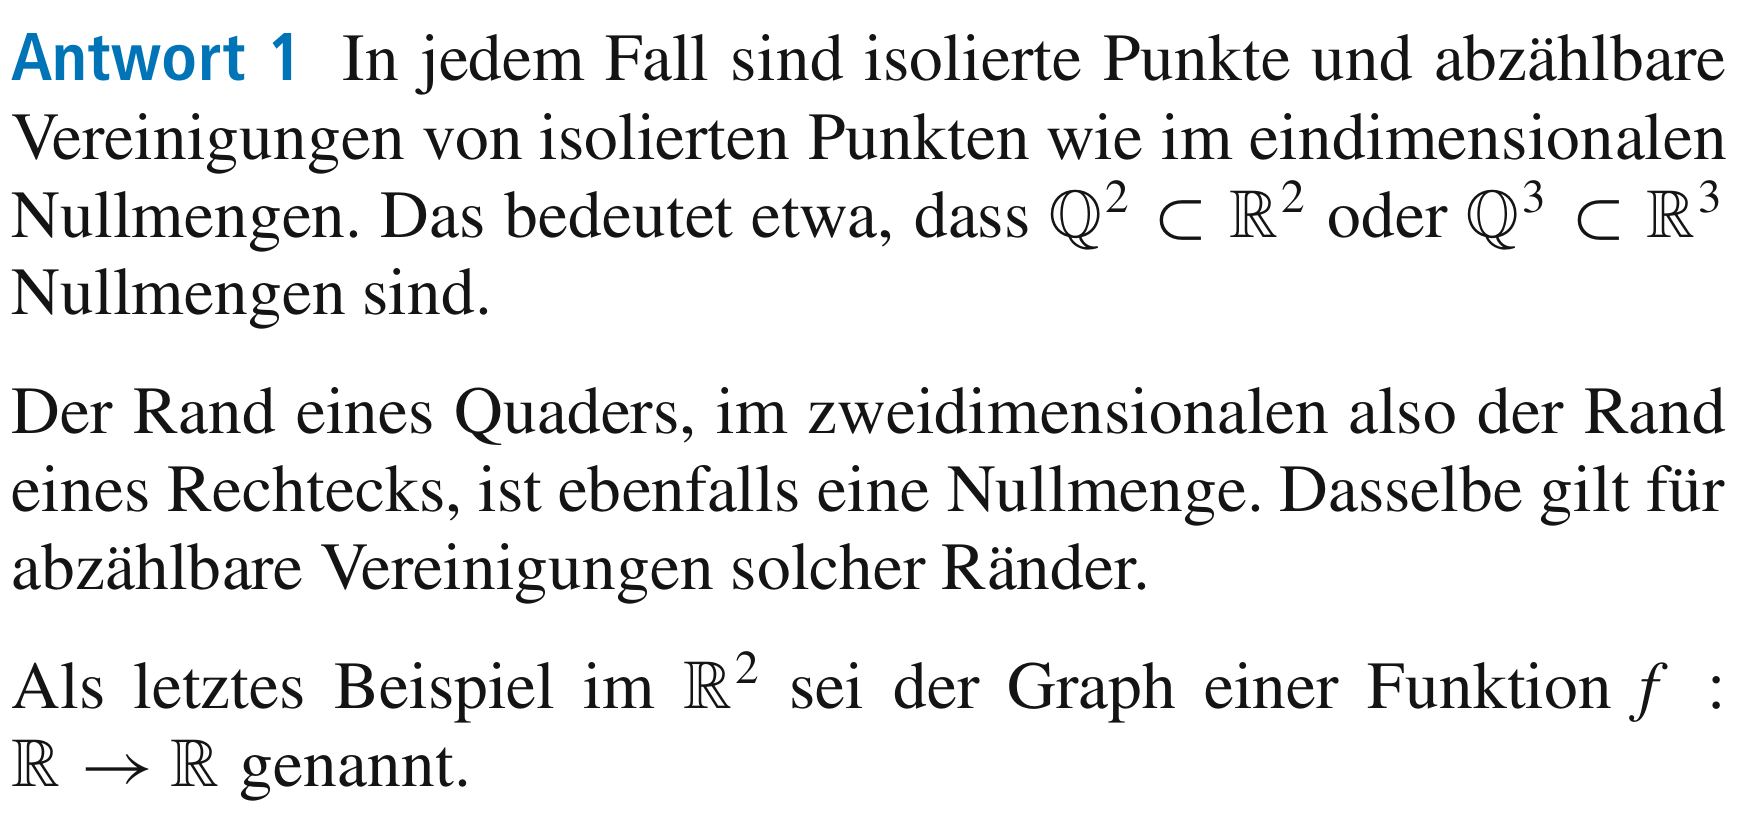
\includegraphics[width=0.8\textwidth]{Dateien/Nullmengen.png}
\end{center}
\end{Beispiel}
\begin{Def}{Fast überall}
Sei $E(x)$ eine Eigenschaft, sodass wir für $\forall x \in \R^n$ wissen, ob die Eigenschaft $E(x)$ erfüllt ist. Wir sagen, dass $E(x)$ \red{fast überall} gilt, wenn die Menge aller Punkte, wo $E(x)$ nicht gilt, eine Nullmenge ist.
\end{Def}
\begin{Beispiel}{Fast überall konstante Funktion}
Sei $f(x)=\begin{cases}42 \mbox{ wenn $x\neq \infty$} \\
\infty \mbox{ wenn $x=\infty$}\end{cases}$. Die Funktion $f(x)$ ist fast überall konstant, außer in einer Nullmenge (also in der Unendlichkeit). 
\end{Beispiel}
Es ist auch nützlich sich zu merken, dass wenn $||f||_1=0$, dann $N=\{ x\in \R^n | f(x)\neq 0\}$ eine nullmenge ist.
\begin{Satz}{Satz}{Modifikationssatz}
Seien $f,g:\R^n\rightarrow \C$ zwei Funktionen, die fast überall gleich sind. Wenn $f$ integrierbar ist, dann ist auch $g$ integrierbar und es gilt $\int f = \int g$.
\end{Satz}
\begin{Satz}{Lemma}{Geometrische Charakterisierung von Nullmengen}
    Ist $N$ eine Nullmenge, so gibt es zu jedem $\epsilon>0$ eine messbare offene Menge $U$ mit $N\subseteq U$ und $v(U)<\epsilon$. \\
    Eine Menge $N\subseteq \R^n$ ist genau dann eine Nullmenge, wenn es zu jedem $\epsilon>0$ abzählbar viele Quader $Q_1, Q_2, ..., Q_n$ gibt, sodass
    $$N\subseteq \bigcup_{k=1}^{\infty}Q_k \mbox{ und }\sum_{k=1}^\infty v(Q_k)>\epsilon$$
\end{Satz}
Eine nützliche, aber nicht so wichtige Eigenschaft ist, dass wenn $f$ integrierbar ist, dann auch $f(x-a)$ integrierbar ist, wenn $a$ in der Definitionsmenge ist.
\newpage
\subsection{Konvergenzsätze}
Zuerst wollen wir uns an die punktweise und gleichmäßige Kovergenz aus MfP2 erinnern.
\begin{Def}
{Gleichmäßige Konvergenz}
Sind $(X,d_X)$ und $(Y,d_Y)$ metrische Räume und $(f_n:X\to Y)_{n\in\mathbb{N}}$ eine Folge von Abbildungen.\\
Wir sagen, dass $f$ genau dann \red{gleichmäßig} gegen eine Grenzfunktion $f$ \red{konvergiert}, wenn es für alle $\epsilon>0$ ein $N=N(\epsilon)\in\mathbb{N}$ gibt, sodass
\begin{equation*}
    d_Y(f_n(x),f(x))<\epsilon\quad \forall n\geq N\land \forall x\in X.
\end{equation*}
\end{Def}
\begin{Def}
{Punktweise Konvergenz}
Eine Folge $(f_n)$ von Abbildungen \red{konvergiert punktweise} gegen eine Abbildung $f$, falls $\lim_{n\to\infty}f_n(x)=f(x)\,\forall x\in X$.
\end{Def}
\begin{Beispiel}
    {Gleichmäßige Konvergenz}
    Wir betrachten die Funktionenfolge
    \begin{equation*}
        f_n(x)=\sqrt{\vert x \vert^2 + \frac{1}{n^2}} \qquad x \in \mathbb{R}.
    \end{equation*}
    Konvergiert diese Folge gleichmäßig gegen eine Grenzfunktion, sagen wir $f(x)=\vert x \vert$? In weiser Voraussicht und um die weitere Rechnung plausibel zu machen, schauen wir uns zunächst die folgende Ungleichung an: 
    \begin{equation*}
        \sqrt{a+b} \leq \sqrt{a+b+2\sqrt{ab}} = \sqrt{(\sqrt{a}+\sqrt{b})^2}=\sqrt{a}+\sqrt{b}.
    \end{equation*} \\
    
    Damit können wir nun recht schnell nachprüfen:
    \begin{align*}
        \forall \epsilon > 0 \,\exists N\in\mathbb{N}\, &\forall x\in D_f \,\forall n\geq N: \\
            &\vert f_n(x)-f(x) \vert = \bigl| \sqrt{\vert x \vert^2 + \frac{1}{n^2}} - \vert x \vert \bigr| \leq \bigl| \vert x \vert + \frac{1}{n} - \vert x \vert \bigr| = \frac{1}{n} \leq \frac{1}{N} < \epsilon
    \end{align*}
    Das Kriterium ist also erfüllt und die Funktion damit gleichmäßig konvergent (und daher auch automatisch punktweise konvergent), da wir die $x$-Abhängigkeit in der Abschätzung losgeworden sind.
\end{Beispiel}
Ebenso ein Beispiel, um uns auf die Quotientenvektorräume aus MfP2 zu erinnern.
\begin{Beispiel}{Quotientenvektorraum}
    Sei $V=\R^4$ und $U=span\{(1,1,0,0)^T, (0,1,-1,0)^T\}\subseteq V$ ein Untervektorraum. Wir sollen zeigen, dass im Quotientenvektorraum $U/V$ gilt
    $$[\begin{pmatrix}
        1 \\
        0 \\
        1 \\
        2 \\
    \end{pmatrix}]=[\begin{pmatrix}
        3 \\
        1 \\
        2 \\
        2 \\
    \end{pmatrix}] \mbox{ und }[\begin{pmatrix}
        1 \\
        0 \\
        1 \\
        0 \\
    \end{pmatrix}]\neq[\begin{pmatrix}
        1 \\
        0 \\
        0 \\
        0 \\
    \end{pmatrix}]$$
    Dabei bezeichnet [$v$] die Äquvialenzklasse von $v\inV$ von $V/U$. \\
    Ein Quotientenvektorraum besteht aus allen Vektoren $a,b\in V$ für die gilt $a+b\in U$.
    $$\begin{pmatrix}
        1 \\
        0 \\
        1 \\
        2 \\
    \end{pmatrix}+\begin{pmatrix}
        3 \\
        1 \\
        2 \\
        2 \\
    \end{pmatrix}=\begin{pmatrix}
        4 \\
        1 \\
        3 \\
        0 \\
    \end{pmatrix}$$
    Wir können nun den Vektor $\begin{pmatrix}
        4 \\
        1 \\
        3 \\
        0 \\
    \end{pmatrix}$ mit den Basisvektoren von $U$ darstellen
    $$\begin{pmatrix}
        4 \\
        1 \\
        3 \\
        0 \\
    \end{pmatrix}= a \begin{pmatrix}
        1 \\
        1 \\
        0 \\
        0 \\
    \end{pmatrix}+b\begin{pmatrix}
        0 \\
        1 \\
        -1 \\
        0 \\
    \end{pmatrix}$$
    Wenn wir $a=4$ und $b=1$ setzen, dann wird das Ungleichungssystem gelöst. Also stimmt die erste Äquivalenzklasse. Nun gucken wir uns das für die anderen zwei Vektoren an
    $$\begin{pmatrix}
        1 \\
        0 \\
        1 \\
        0 \\
    \end{pmatrix}+\begin{pmatrix}
        1 \\
        0 \\
        0 \\
        0 \\
    \end{pmatrix}=\begin{pmatrix}
        2 \\
        0 \\
        1 \\
        0 \\
    \end{pmatrix} \mbox{,     } \begin{pmatrix}
        2 \\
        0 \\
        1 \\
        0 \\
    \end{pmatrix}=a \begin{pmatrix}
        1 \\
        1 \\
        0 \\
        0 \\
    \end{pmatrix}+b\begin{pmatrix}
        0 \\
        1 \\
        -1 \\
        0 \\
    \end{pmatrix}$$
    Und wir merken schon, dass es keine $a$ und $b$ gibt, sodass das Gleichungssystem gelöst werden kann, daher gehören die letzten zwei Vektoren nicht zu der Äquvivalenzklasse.
\end{Beispiel}
Nun kommen wir zu sehr wichtigen Sätzen.
\begin{Satz}{Theorem}{Satz von Riesz-Fischer}
    Vorausgesetzt $f_k$ ist eine $\mathcal{L}^1$-Cauchy-Folge integrierbarer Funktionen, dann \begin{itemize}
        \item existiert $f\in \mathcal{L}^1(\R^n)$ mit $\lim_{k\rightarrow \infty}f_k = f$ mit $\int f dx = \lim_{k\rightarrow \infty}\int f_k dx$ und
        \item $(f_k)$ konvergiert punktweise gegen $f$.
    \end{itemize}
    Somit ist $\mathcal{L}^1(\R^n)$ ein Banachraum. Die \red{Vertauschbarkeit} von Integral und Limes folgt grob aus der Konvergenz bzgl. der $\mathcal{L}^1$-Halbnorm.
\end{Satz}
Beachtet, dass der $\mathcal{L}^1$- Grenzwert nicht eindeutig ist, aber es kann sein, dass sich die Grenzwerte nur auf eine Nullmenge unterscheiden.
\begin{Satz}{Satz}{Satz von Beppo-Levi von der monotonen Konvergenz}
    Voraussetzungen:
    \begin{itemize}
        \item $f_k:\R^n\rightarrow \R \cup \{ \infty\}$ ist monoton wachsende/fallende Folge integrierbarer Funktionen
        \item $f_k$ konvergiere punktweise gegen $f(x)=\lim_{k\rightarrow \infty} f_k(x)$
        \item Die Folge $\int f_k dx$ der Integrale ist beschränkt.
    \end{itemize}
    Dann folgt, dass $f$ integrierbar ist und dass $\int f dx = \lim_{k\rightarrow \infty} \int f_k dx$
\end{Satz}
\begin{Satz}{Satz}{Satz von Lebesgue von der majorisitierten Konvergenz}
    Voraussetzungen:
    \begin{itemize}
        \item $f_k:\R^n\rightarrow \C \cup \{ \infty\}$ ist eine Folge integrierbaren Funktionen
        \item $f_k$ konvergiert fast überall punktweise gegen eine Funktion $f$
        \item Es gibt eine integrierbare Majorante $F$ mit $|f_k|\leq F$ für $\forall k$.
    \end{itemize}
    Dann folgt, dass $f$ integrierbar ist und dass $\int f dx = \lim_{k\rightarrow \infty} \int f_k dx$
\end{Satz}
\begin{Beispiel}{Satz von integrierbaren Majoranten angewandt}
    Wir betrachten die Funktion
    $$\delta_n(x)=\begin{cases}
        xn^2 & 0\leq x< \frac{1}{n} \\
        2n-xn^2 & \frac{1}{n} \leq x \leq \frac{2}{n} \\
        0 & \mbox{sonst}
    \end{cases}$$
    Die Funktionenfolge ist unbeschränkt wie wir gesehen haben, da
    $$\max_{x\in\R} \delta_n(x)=n$$
    Es gibt also keine integrierbare Majorante und somit ist nicht sichergestellt, dass Integral und Limes vertauschen zu können. Tatsächlich gilt:
    $$\lim_{n\rightarrow \infty} \int_\R \delta_n(x) dx = 1 \mbox{ und } \int_\R \delta(x)dx = 0$$
\end{Beispiel}
\begin{Beispiel}{Und noch ein Beispiel}
    \begin{center}
    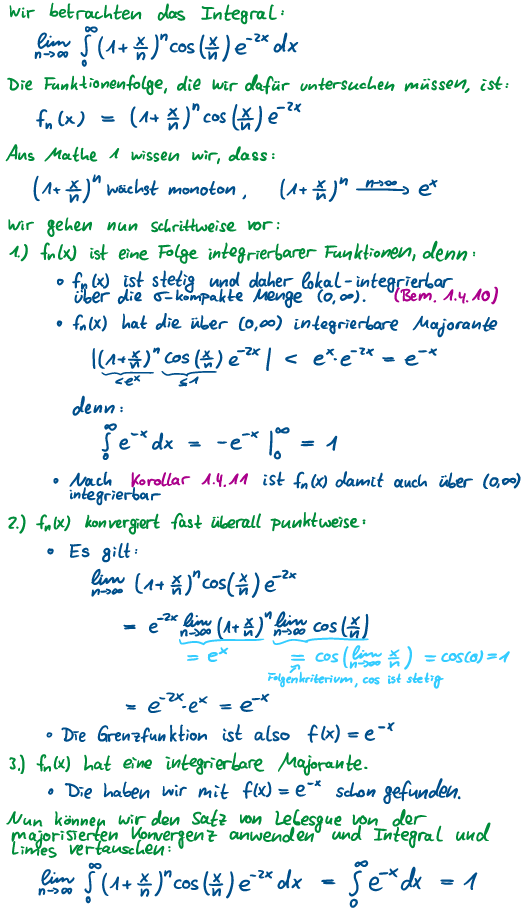
\includegraphics[width=0.80\textwidth]{Dateien/Beppo_Levi_Beispiel.png}
\end{center}
\end{Beispiel}
\newpage
\subsection{Parameterabhängige Integrale}
Die Vertauschbarkeit von Integral und Limes führt zu weiteren, sehr praktischen Sätzen.
\begin{Satz}{Satz}{Verallgemeineter Hauptsatz der Differential- und Integralrechnung}
Voraussetzungen:
\begin{itemize}
    \item $f$ ist differenzierbar auf dem kompakten Intervall $[x_0, x]$.
    \item Die Ableitung von $f$ ist beschränkt.
\end{itemize}
Daraus folgt, dass $f'$ Lebesgue-integrierbar ist über $[x_0, x]$ und dass $$f(x)-f(x_0)=\int_{[x_0, x]} f'(t)dt$$.
\end{Satz}
\begin{Satz}{Satz}{Stetigkeitssatz}
    Voraussetzungen:
    \begin{itemize}
        \item Sei $X$ ein metrischer Raum und $T\subseteq \R^p$
        \item $f:X\times T\rightarrow \C, (x,t)\longmapsto f(x,t)$ ist für feste $x$ über $T$ integrierbar
        \item Für feste $t$ ist die Funktion $x\longmapsto f(x,t)$ stetig
        \item Es gibt eine integrierbare Majorante $\Phi: T\rightarrow \R$, sodass $|f(x,t)|\leq \Phi(t)$ für $\forall (x,t)\in X\times T$.
    \end{itemize}
    Daraus folgt, dass $F(x)=\int_T f(x,t)dt$ ist auf $X$ stetig.
\end{Satz}
\begin{Satz}{Satz}{Differentiationssatz}
        Voraussetzungen:
    \begin{itemize}
        \item Sei $X\subseteq \R^n$ und $T\subseteq \R^p$
        \item $f: X\times T\rightarrow \C$, $(x,t)\rightarrow f(x,t)$ ist für feste $x$ über $T$ integrierbar
        \item Für feste $t$ ist die Funktion $x\longmapsto f(x,t)$ stetig diff'bar
        \item Es gibt eine intergierbare Majorante $\Phi:T\rightarrow \R$ mit
        $$|\frac{\partial f}{\partial v_\mu}(x,t)|\leq \Phi(t)\mbox{ für }\forall (x,t)\in X\times T\mbox{ für }\mu = 1,...,n$$
    \end{itemize}
    Daraus folgt, dass
    \begin{itemize}
        \item $F(x)=\int_T f(x,t)dt$ ist stetig diff'bar,
        \item $t\mapsto\frac{\partial}{\partial x_p}f(x,t)$ ist für jedes $x$ integrierbar und
        \item es gilt $\frac{\partial}{\partial x_\mu}\int_T f(x,t)dt=\int_T \frac{\partial}{\partial x_\mu} (x,t) dt$.
    \end{itemize}
\end{Satz}
\begin{Beispiel}{Fourier-Transformation}
        \begin{center}
    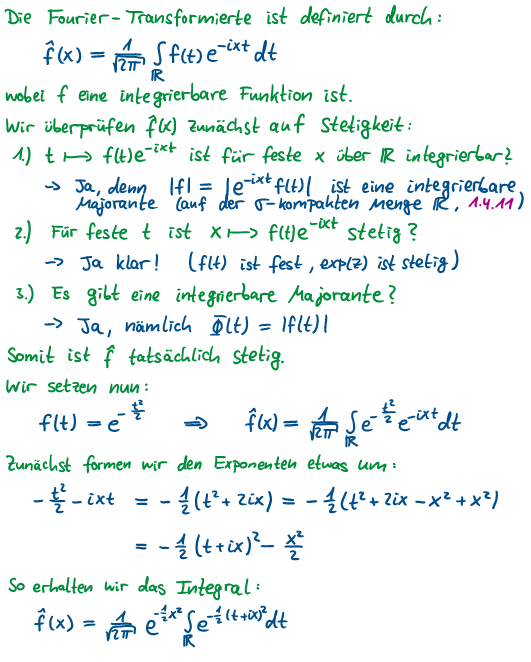
\includegraphics[width=0.80\textwidth]{Dateien/Fourier_Transform_1.png}
    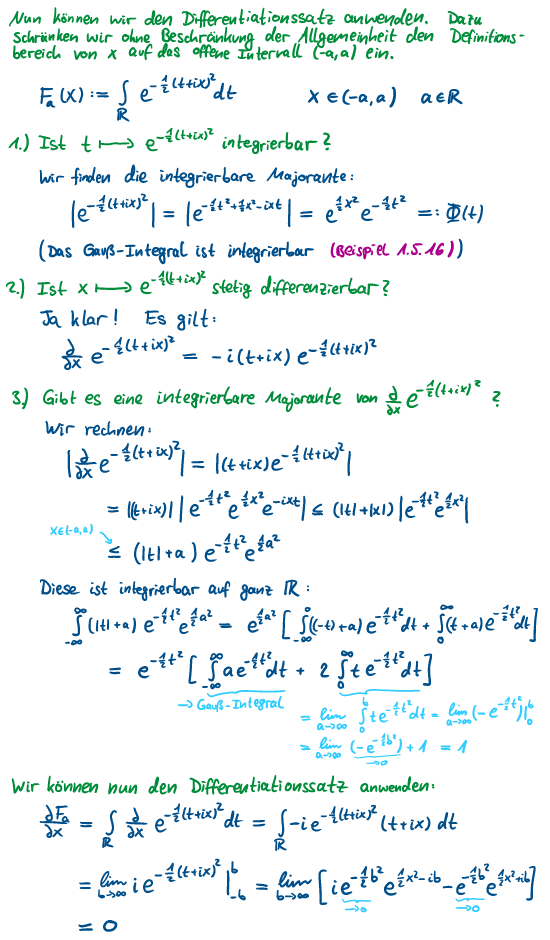
\includegraphics[width=0.80\textwidth]{Dateien/Fourier_Transform_2.png}
    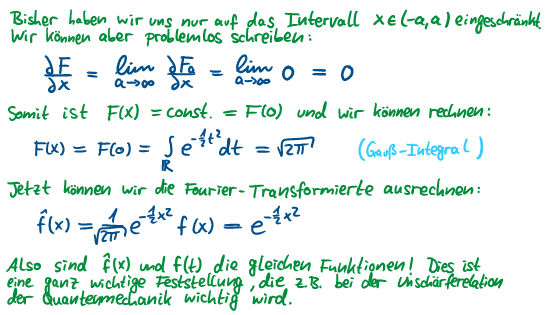
\includegraphics[width=0.80\textwidth]{Dateien/Fourier_Transform_3.png}
\end{center}
\end{Beispiel}
\newpage
Aus all diesen Sätzen kommt nun der Höhepunkt der Integrationstheorie. Die folgenden zwei Sätze sind von enormer bedeutung in der Physik, also merkt sie euch. 
\begin{Satz}{Satz}{Satz von Tonelli}
    Vorausgesetzt $f:\R^p\times \R^q \rightarrow \C$ ist fast überall stetig oder lokal integrierbar. Dann gilt die folgende Äquivalenz
    $$\int_{\R^q}(\int_{\R^p} |f(x,y)|dx)dy \quad\mbox{oder}\quad\int_{\R^p}(\int_{\R^q} |f(x,y)|dx)dy\mbox{ existiert} $$
    $$\iff \mbox{$f$ ist über $\R^p\times\R^q$ integrierbar}$$
\end{Satz}
\begin{Satz}{Satz}{Transformationssatz}
    Voraussetzung:
    \begin{itemize}
        \item $U,V\subseteq \R^n$ offen
        \item $T: U\rightarrow V$ ist ein Diffeomorphismus
        \end{itemize}
        Daraus folgen
    \begin{itemize}
            \item die Äquivalenz $f:V\rightarrow \C\cup\{\infty\}$ integrierbar $\iff f\circ T\cdot |\det(dT)|$ integrierbar
            \item $\int_u f(T(x))|\det(dT)|dx=\int_V f(y)dy$
        \end{itemize}
    
\end{Satz}
Zur Erinnerung die definition der allgemeinen linearen Gruppe: $$GL(n,\R)=\{A\in \mbox{Mat}(n,\R)| \det(A)\neq0\}$$
Außerdem nicht vergessen, dass der Betrag der Determinante einer Matrix das gerichtete Volumen eines Parallelepipeds darstellt.
\begin{Def}{Affine Transformationen}
    Voraussetzung:
    \begin{itemize}
        \item $T:\R^n\rightarrow \R^n$, $T(x)=Ax+b$ mit $A\in GL(n,\R), b\in \R^n$
        \item $f:K\rightarrow \C$ ist über $K\subseteq \R^n$ integrierbar
    \end{itemize}
    Daraus folgen
    \begin{itemize}
        \item $dT=A \Rightarrow \det(dT)=\det(A)\in \R/\{0\}$
        \item $f\circ T$ ist über $T^{-1}(K)$ integrierbar
        \item Es gilt $\int_{T^{-1}(K)} f(T(x)) dx = \frac{1}{|\det(A)|}\int_K f(y) dy$.
    \end{itemize}
\end{Def}
\begin{Beispiel}{Präsenzaufgabe 1 aus dem Blatt 6}
    \red{WIP}
\end{Beispiel}
\begin{Beispiel}{Bestimmung eines uneigentlichen Integrals}
    \begin{center}
    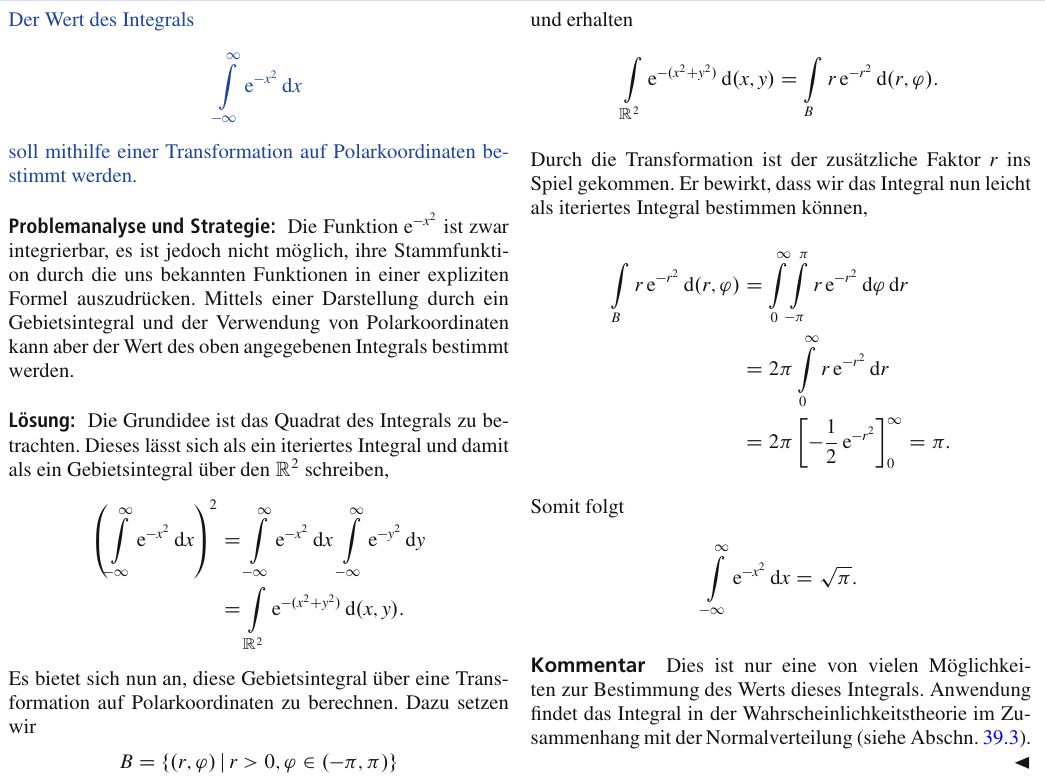
\includegraphics[width=0.95\textwidth]{Dateien/Uneigentlich_e_hoch_x_quadrat.png}

\end{center}
\end{Beispiel}
\begin{Beispiel}{Transformationssatz im Einsatz}
            \begin{center}
    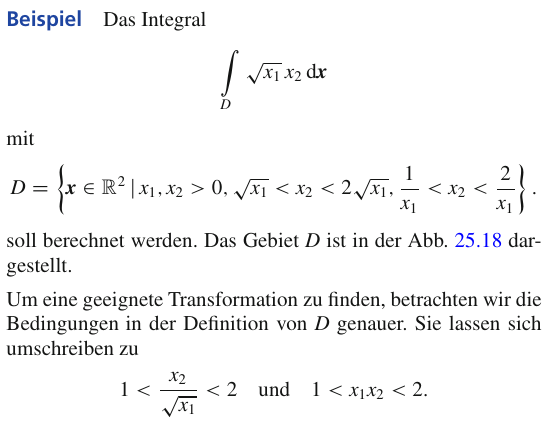
\includegraphics[width=0.52\textwidth]{Dateien/Transformationssatz1.png}
    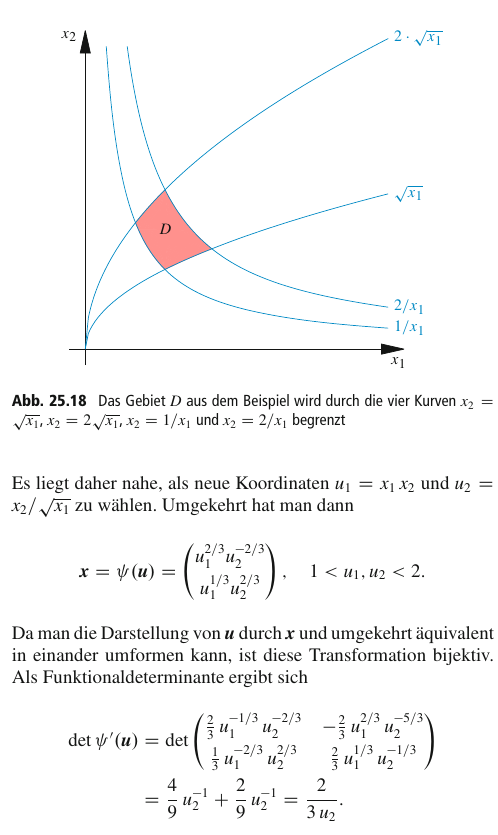
\includegraphics[width=0.52\textwidth]{Dateien/Transformationssatz2.png}
    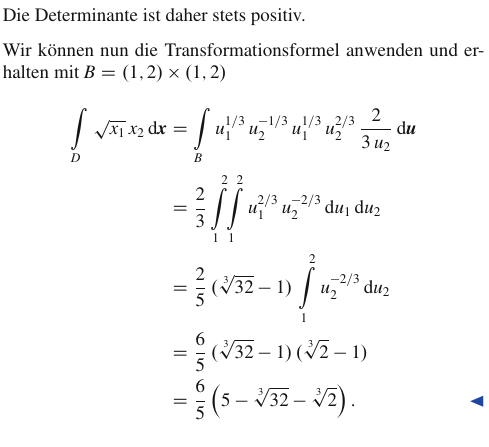
\includegraphics[width=0.52\textwidth]{Dateien/Transformationssatz3.png}
\end{center}
\end{Beispiel}
\newpage
\subsection{Exkurs: Wichtige Koordinatensysteme}
Dieses Thema ist euch allen schon aus der Physik 2 bekannt und könnt es überspringen, aber guck euch die Beispiele zur Erinnerung vor der Klausur nochmal an. \\
Für das \red{Polarkoordinatensystem} gelten die folgenden Gleichungen:
$$x_1=r\cos(\varphi)$$
$$x_2=r\sin(\varphi)$$
$$\Phi(r, \varphi) = \begin{pmatrix}
    r\cos(\varphi) \\
    r\sin(\varphi)
\end{pmatrix}$$
\begin{Def}{Integration mit Polarkoordinaten}
Ist $D\subseteq \R^2, f\in L(D)$ und $B$ die Beschreibung von $D$ durch Polarkoordinaten, so gilt
$$\int_D f(x_1,x_2)d(x_1,x_2) = \int_B f(r\cos(\varphi), r\sin(\varphi))rd(r, \varphi)$$
\end{Def}
\begin{Beispiel}{Integration mit Polarkoordinaten}
\begin{center}
    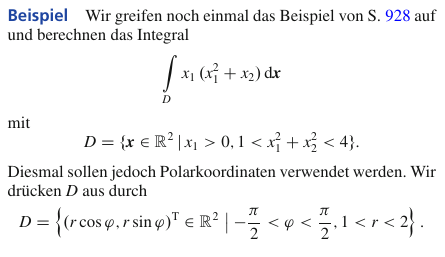
\includegraphics[width=0.52\textwidth]{Dateien/Polarkoord1.png}
    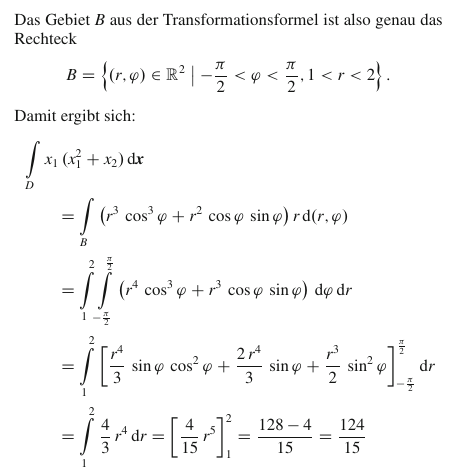
\includegraphics[width=0.52\textwidth]{Dateien/Polarkoord2.png}
\end{center}
\end{Beispiel}

Für das \red{Zylinderkoordinatensystem} gelten die folgenden Gleichungen:
$$x_1=\rho\cos(\varphi)$$
$$x_2=\rho \sin(\varphi)$$
$$x_3=z$$
$$\Phi(\rho, \varphi, z)=\begin{pmatrix}
    \rho \cos(\varphi) \\
    \rho \sin(\varphi) \\
    z
\end{pmatrix}$$
\begin{Def}{Integration mit Zylinderkoordinaten}
Ist $D\subseteq \R^3, f\in L(D)$ und $B$ die Beschreibung von $D$ durch Polarkoordinaten, so gilt
$$\int_D f(x_1,x_2,x_3)d(x_1,x_2,x_3) = \int_B f(\rho\cos(\varphi), \rho\sin(\varphi),z)\rho d(\rho, \varphi, z)$$
\end{Def}
\begin{Beispiel}{Integration mit Zylinderkoordinaten}
    \begin{center}
    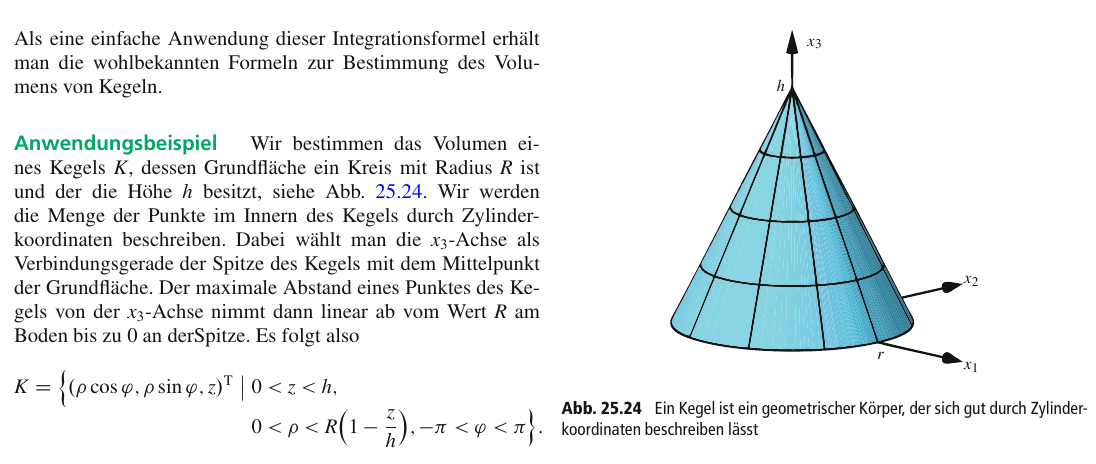
\includegraphics[width=1.0\textwidth]{Dateien/Zylinderkoord1.png}
    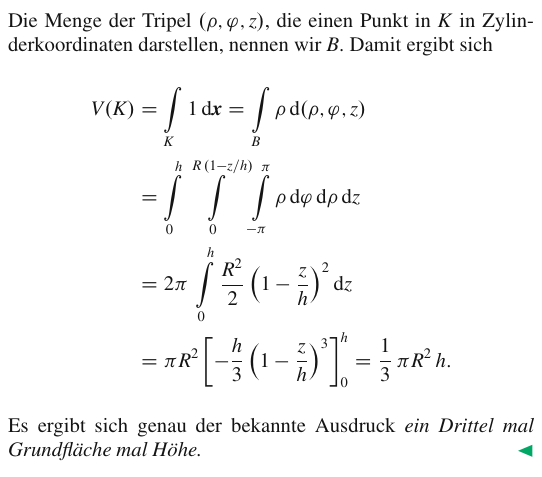
\includegraphics[width=0.7\textwidth]{Dateien/Zylinderkoord2.png}
\end{center}
\end{Beispiel}
Zum guten Letzt gelten für das \red{Kugelkoordinatensystem} die folgenden Gleichungen:
$$x_1=r\cos(\varphi)\sin(\theta)$$
$$x_2=r \sin(\varphi)\sin(\theta)$$
$$x_3=z\cos(\theta)$$
$$\Phi(r, \varphi, \theta)=\begin{pmatrix}
    r \cos(\varphi)\sin(\theta) \\
    r \sin(\varphi)\sin(\theta) \\
    r \cos(\theta)
\end{pmatrix}$$
\begin{Def}{Integration mit Kugelkoordinaten}
Ist $D\subseteq \R^3, f\in L(D)$ und $B$ die Beschreibung von $D$ durch Polarkoordinaten, so gilt
$$\int_D f(x_1,x_2,x_3)d(x_1,x_2,x_3) = \int_B f(r \cos(\varphi)\sin(\theta), r \sin(\varphi)\sin(\theta),r \cos(\theta))r^2\sin(\theta) d(r, \varphi, \theta)$$
\end{Def}
\begin{Beispiel}{Integration mit Kugelkoordinaten}
        \begin{center}
    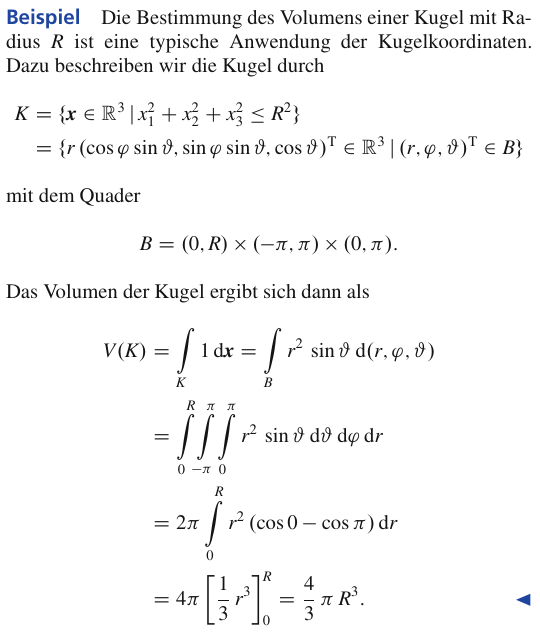
\includegraphics[width=0.7\textwidth]{Dateien/Kugelkoord.png}
\end{center}
\end{Beispiel}